\documentclass{ximera}

%\addPrintStyle{..}

\begin{document}
	\author{Bart Lambregs}
	\xmtitle{Inleiding}{}
    \xmsource\xmuitleg

	Als we in een vlak bewegen, hebben we te maken met een tweedimensionale beweging. 
	Ten opzichte van een referentiestelsel met twee assen, kunnen we de beweging beschrijven.
	\begin{image}
		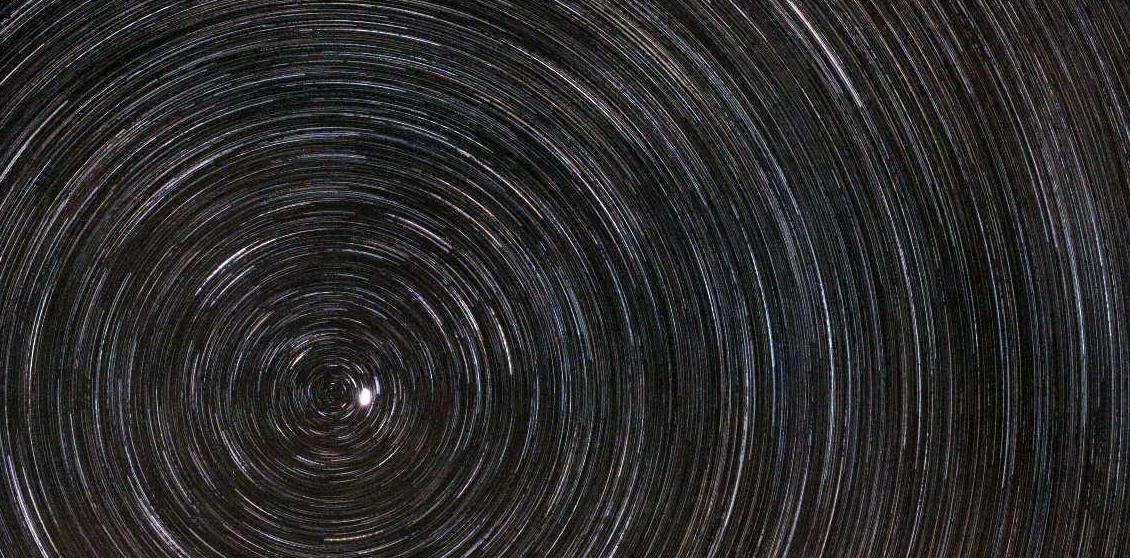
\includegraphics[width=.7\textwidth]{sterrentrajecten}
	\end{image}
	\captionof{figure}{Sterrentrajecten aan de hemel}
	We behandelen twee concrete bewegingen in dit hoofdstuk, de horizontale worp en de eenparig cirkelvormige beweging.
	
\end{document}

% \todo{Hoe zit het met poolcoördinaten? Die zijn niet te gebruiken als referentiestelsel \ldtos?}